\documentclass[prb,preprint]{revtex4-1} 
% The line above defines the type of LaTeX document.
% Note that AJP uses the same style as Phys. Rev. B (prb).

\usepackage{amsmath}  % needed for \tfrac, \bmatrix, etc.
\usepackage{amsfonts} % needed for bold Greek, Fraktur, and blackboard bold
\usepackage{graphicx} % needed for figures
\usepackage{tabularx}
\usepackage{color}

\begin{document}

\title{Optical Pumping of Rubidium 85 and 87}
% In a long title you can use \\ to force a line break at a certain location.

\author{Yumeng Melody Cao}
\email{mcao@smith.edu} 
\affiliation{Department of Physics, Smith College, Northampton, MA 01063}
\author{He Claudia Yun}
\email{hyun@smith.edu}
\affiliation{Department of Physics, Smith College, Northampton, MA 01063}

% See the REVTeX documentation for more examples of author and affiliation lists.

\date{\today}

%____________abstract____________________________________________

\begin{abstract}


When an external static magnetic field is applied to an atom, the hyperfine energy levels of the atom split, with spacing proportional to the magnitude of that field. This is called the Zeeman effect. Optical pumping of Rubidium is used in this experiment to examine this effect. A circularly polarized laser beam with wavelength of 794.8 nm was directed through Rubidium vapor surrounded by Helmholtz coils in all three dimensions, and detected by a photodiode. A radio frequency (RF) signal was applied to the Rb vapor. When changing the magnitude of the magnetic field created by the Helmholtz coil, the opacity of the Rb vapor would have a sudden increase when the external field was in resonance with the RF signal due to a stronger absorption. Varying the RF signal, we observed a change in the magnitude of the resonant field. From the relationship between the signal and the field, the Lande g-factor was determined for $^8$$^5$Rb, $g_{85}=0.34\pm0.0002$, and $^8$$^7$Rb, $g_{87}=0.51\pm0.0004$, whose theoretical values are 1/3 and 1/2 respectively. \\

\end{abstract}

\maketitle 

%____________Introduction____________________________________________
\section{Introduction}

%\textcolor{blue}{in the interests of time, I'm not making detailed comments on the Introduction}

In quantum mechanics, hydrogen-like atoms, i.e. atoms with only one valence electron, are modeled such that the outmost electron can only exist in some discrete energy levels. These orbits are described by quantum numbers $n$ and $l$, where $n=1, 2, ...$ and $l=s, p, d, f, ...$, denoting the energy and orbital angular momentum of the electron. However, this model does not consider the spin of the electron. When the spin is taken into account, each energy level will split into two due to the coupling effect between the spin and the orbital angular momentum of the electron. This is known as the fine structure. The summation $J=L+S$ is the total angular momentum, where $S$ is the electron spin and $L$ is the orbital angular momentum. If the spin of the nucleus $I$ is also considered, each fine-structure level will again split. And the atom will have a total angular momentum $F=I+J$. This is also known as the hyperfine structure. Finally, when a relatively weak external magnetic field is applied, each $F$ level splits into different $M$ levels with spacing proportional to the strength of the field. This splitting is known as the Zeeman effect. The Zeeman splitting is given by

\begin{equation}
E_{z}=g_{F} \mu_{0} BM
\label{zeeman}
\end{equation}

Where $E_{z}$ is the Zeeman energy, the energy difference between two different $M$ levels, B is the external magnetic field strength, and $\mu_{0}$ is the Bohr magneton. From Eq. \eqref{zeeman} it can be seen that $E_{z}$ is linearly proportional to $B$. By changing the RF signal, which will match $E_{z}$, and the magnetic field $B$, we could find out the coupling constant $g_{F}$ for Rubidium.\\

\textcolor{blue}{this suggests that the fractional uncertainty in g will depend on the fractional uncertainties in B and in E}: $ \frac{\delta g}{g} = \sqrt{{\left( \frac{\delta B}{B}\right)}^2 + {\left( \frac{\delta f_{RF}}{f_{RF}}\right)}^2}$ \textcolor{blue}{based on equation 7}

\textcolor{magenta}{are you sure this calculation of uncertainty gives you a fractional uncertainty in g of only 0.0001 (0.01 \%)? That would require knowing both B and f to better than 0.01 \%! How small a fractional change in frequency is possible using this oscillator? What about the factor of 30 in conversion from V to I for the magnet coil? Do you know that to 0.01\%?  And how well do you think you corrected for the zero field offset of approximately 0.2 Gauss (20 microtesla)? Isn't that on the order of your maximum horizontal magnet field in Fig 5? I recommend giving this a closer look so you can come  up with an more accurate estimate of uncertainty in g. This is important, because your deviation in gF for 85Rb is just 3\% (compared to theory) and your deviation for 87Rb is 2\%. A 1\% error in the zero field offset correction plus a 1\% error in the I to V conversion factor (approximately 30?) would give a 2\% error in B just by themselves. } 


\begin{equation}
\mu_{0}=\frac{e\hbar}{2m_{e}}=9.27\times10^{-24} J/T
\label{mu0}
\end{equation}

And $g_{F}$ is the coupling constant, known as the Lande g-factor. 

\begin{equation}
g_{F}=g_{J} \frac{F(F+1)+J(J+1)-I(I+1)}{2F(F+1)}
\label{gf}
\end{equation}
and
\begin{equation}
g_{J}=1+\frac{J(J+1)+S(S+1)-L(L+1)}{2J(J+1)}
\label{gj}
\end{equation}

\begin{figure}[h]
\centering
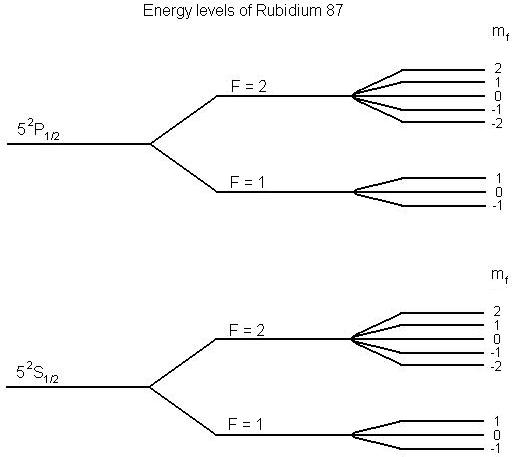
\includegraphics[width=10cm]{energylevels.jpg}
\caption{Zeeman splitting of Rubidium 85 atom \cite{energy}}
\label{energylevels}
\end{figure}

Fig. \ref{energylevels} shows the Zeeman splitting of a Rubidium 87 atom. \\

When a photon with the right energy to excite the electron from level $1s$ to $2p$ enters the atom, the hyperfine levels are so close together that there is an equal possibility of the electron landing in any $F$ level with any $M$. However, there are certain rules the electron has to follow, one of which is that the electron's $M$ value cannot be altered by more than 1. This is to say, $\Delta M=-1, 0, 1$. $\Delta M$ is decided by the nature of the photon. When the applied magnetic field is parallel to the direction of propagation of the photon, a right-circularly-polarized photon will always give $\Delta M=1$ and a left-circularly-polarized photon will give $\Delta M=-1$. The rule also applied to emission. For example, when the electron falls from $2p$ back to $1s$, $\Delta M$ is equally likely to be 1, 0, and -1, so the average $\Delta M=0$. \\

In out experiment, a right-circularly-polarized laser beam with the right frequency to excite electrons from ground state to first excited state passes through some Rubidium vapor and is then detected by a photodiode. Because of the polarization of the photons, transitions induced all have $\Delta M=1$. The average emissions have average $\Delta M=0$, so very quickly all the electrons will be "pumped" up to the highest $M$ level. When that happens, the Rubidium vapor is unable to absorb any more photon, which means that it has become transparent to the laser beam. Then an RF (Radio Frequency) signal is introduced into the system. When the RF signal has the exact energy between the Zeeman splitting, it "depumps" the electrons from the highest $M$ level down, and the Rubidium vapor can absorb photons again, which will cause a sudden decrease in the intensity of the laser beam detected by the photodiode. \\

%____________Experiment____________________________________________
\section{Experiment}

To implement the optical pumping process, we used the apparatus shown in Fig. 
\ref{exp}, manufactured by TeachSpin Inc \cite{teach}. \\

\begin{figure}[h]
\centering
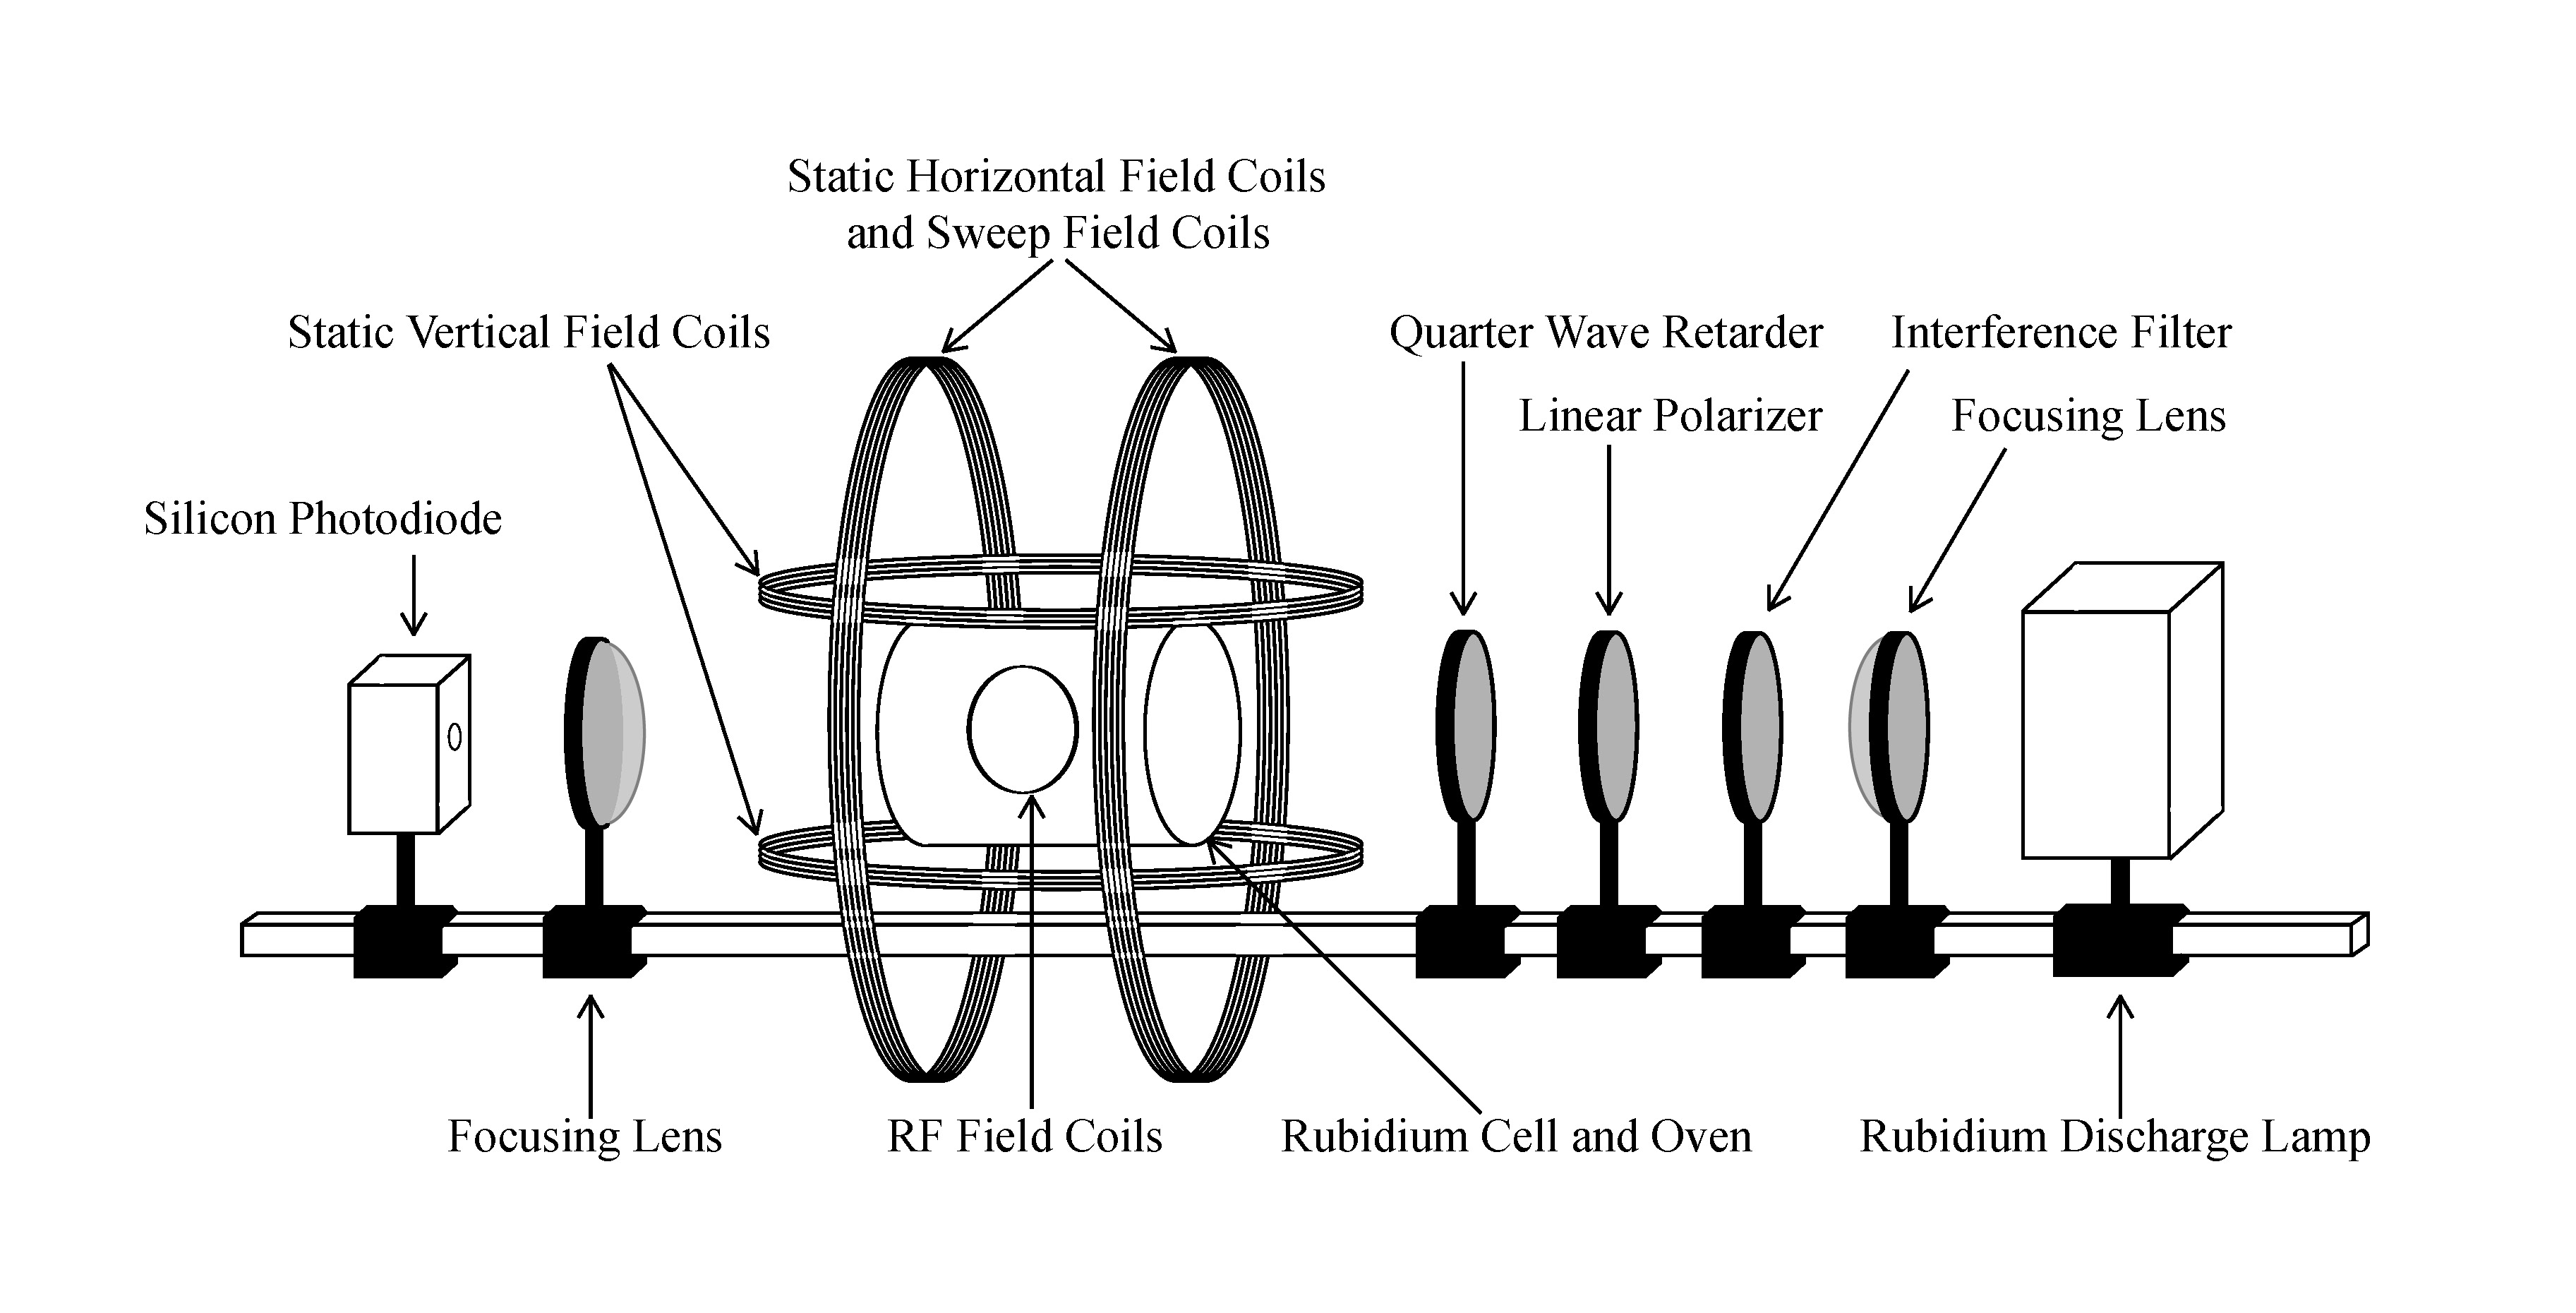
\includegraphics[width=16cm]{exp.jpg}
\caption{Optical pumping of Rubidium apparatus including the labelled components \cite{rib}. There are three main components to this optical pumping set up on the optical rail. The light source (right hand side), the rubidium cell in the center (kept at 50$^{\circ}$C) surrounded by Helmholtz and RF field coils (center) and the detector (left hand side). }
\label{exp}
\end{figure}


Light is emitted from a rubidium lamp on the right side of the optical rail with a wavelength of 794.8 nm with an energy of 1.56 eV; the light itself is purple to the visible eye.  the interference filter limits the bandwidth of light with a pass band of 790 nm to 830 nm, and the linear polarizer and quarter wave retarder convert the light from random polarization to circular polarization. The circular polarized light mandates only $\Delta M=+1$ electric dipole transitions in the atom.\\

The circularly polarized photos next enter the temperature controlled (50$^{\circ}$C) rubidium cell containing both isotopes of rubidium,   $^8$$^5$Rb and $^8$$^7$Rb. The Helmholtz coils provide the magnetic fields, are driven by dial controlled variable voltage dividers, and are monitored by the x-axis input of the oscilloscope. The RF field coils are driven by a function generator and drive the sample out of the optically pumped state when the sweep field is at resonant with the energy difference between two neighbor levels.\\

The left side of the optical rail measures the intensity of light passing through the sample which in effect allows us to see when the sample is driven out of the optically pumped state. This signal detected by the photodiode is monitored by the y-axis input of the oscilloscope. \\

In the beginning of the experiment, we removed the quarter wave retarder and the linear polarizer to align the setup by moving the filters and focusing lenses so that the photodiode voltage reading is maximum. Then we put back two linear polarizers, one at either side of the cell, and aligned the two polarizers at 90$^{\circ}$ so that the photodiode voltage reads zero. The quarter wave retarded was then added back and rotated until the photodiode voltage reads a maximum value.\\

%When there is zero field applied by the coils, we know the Earth's magnetic field will have an influence on the Zeeman splitting by allowing atoms to be pumped into the less absorbent stats. So to take into consideration this zero field,

The Earth has a non-zero magnetic field, which would affect Zeeman splitting, therefore we want it to be minimized. We first oriented the apparatus so that the light beam passing through the rubidium cell was aligned along the north-south axis to cancel out the local component of the Earth's magnetic field. The set of vertical Helmholtz coils were used to cancel the vertical component of the earth's field. Now all is left is the horizontal component of the Earth's magnetic field that will be in the opposite direction of the current in the horizontal Helmholtz coils (along the axis of the path of light).When the net field at the cell is zero (applied field and Earth's field are equal and opposite), the Zeeman levels become degenerate and we can no longer pump the atoms into less absorbing states, thus we see a district dip in the line of the oscilloscope in the y-axis connected to the photodiode.\\

Now the apparatus is properly set up, 10 sets of data for the RF frequency ranging from 10 to 100 kHz are taken, in increments of 10kHz. For each data set, the horizontal magnetic field sweep is set so that the time was 100 second, range was at 4.4 and start field at 2 on the nob.This way we could fit all the dips on the scale at all 10 different frequencies.\\


%____________Results____________________________________________
\section{Results}

A series of plots of photodiode voltage versus horizontal sweep voltage are obtained at different RF frequency. \\

\begin{figure}[h!!!!!!!!]
\centering
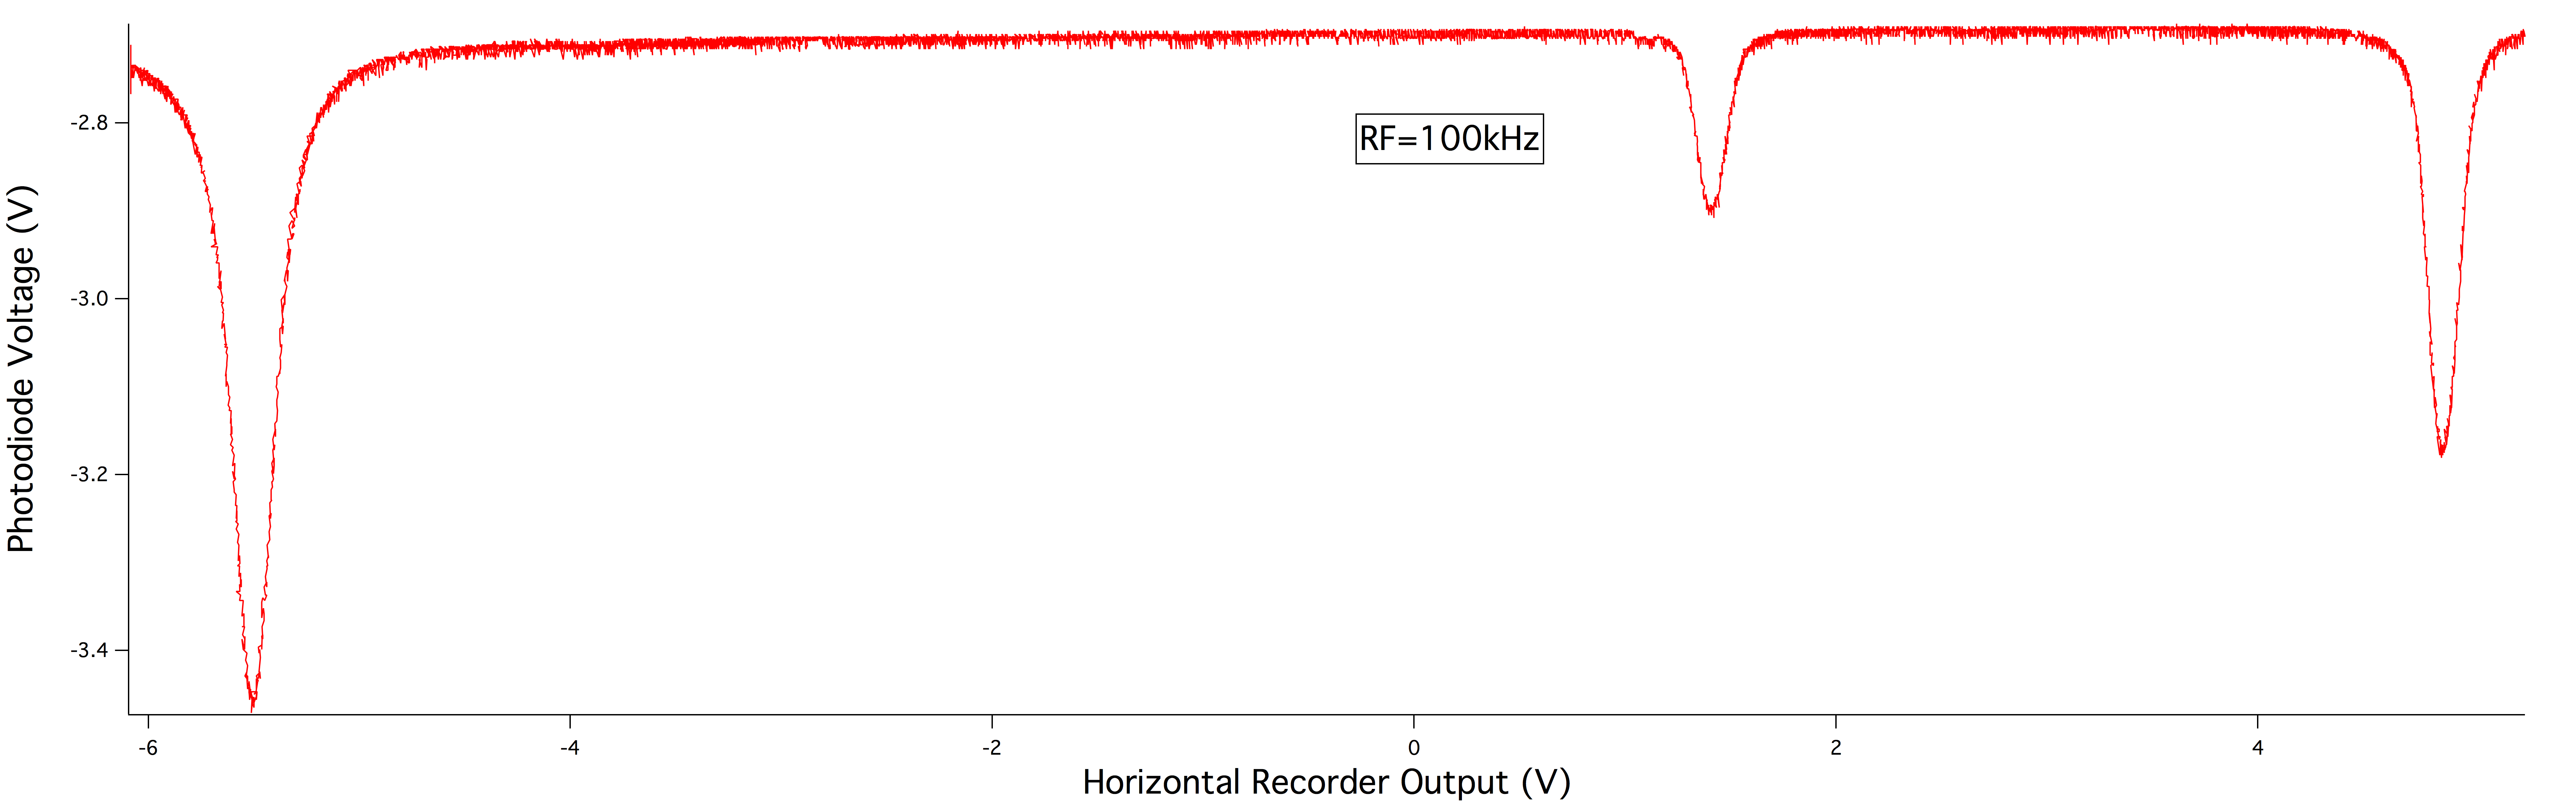
\includegraphics[width=15cm]{100k.png}
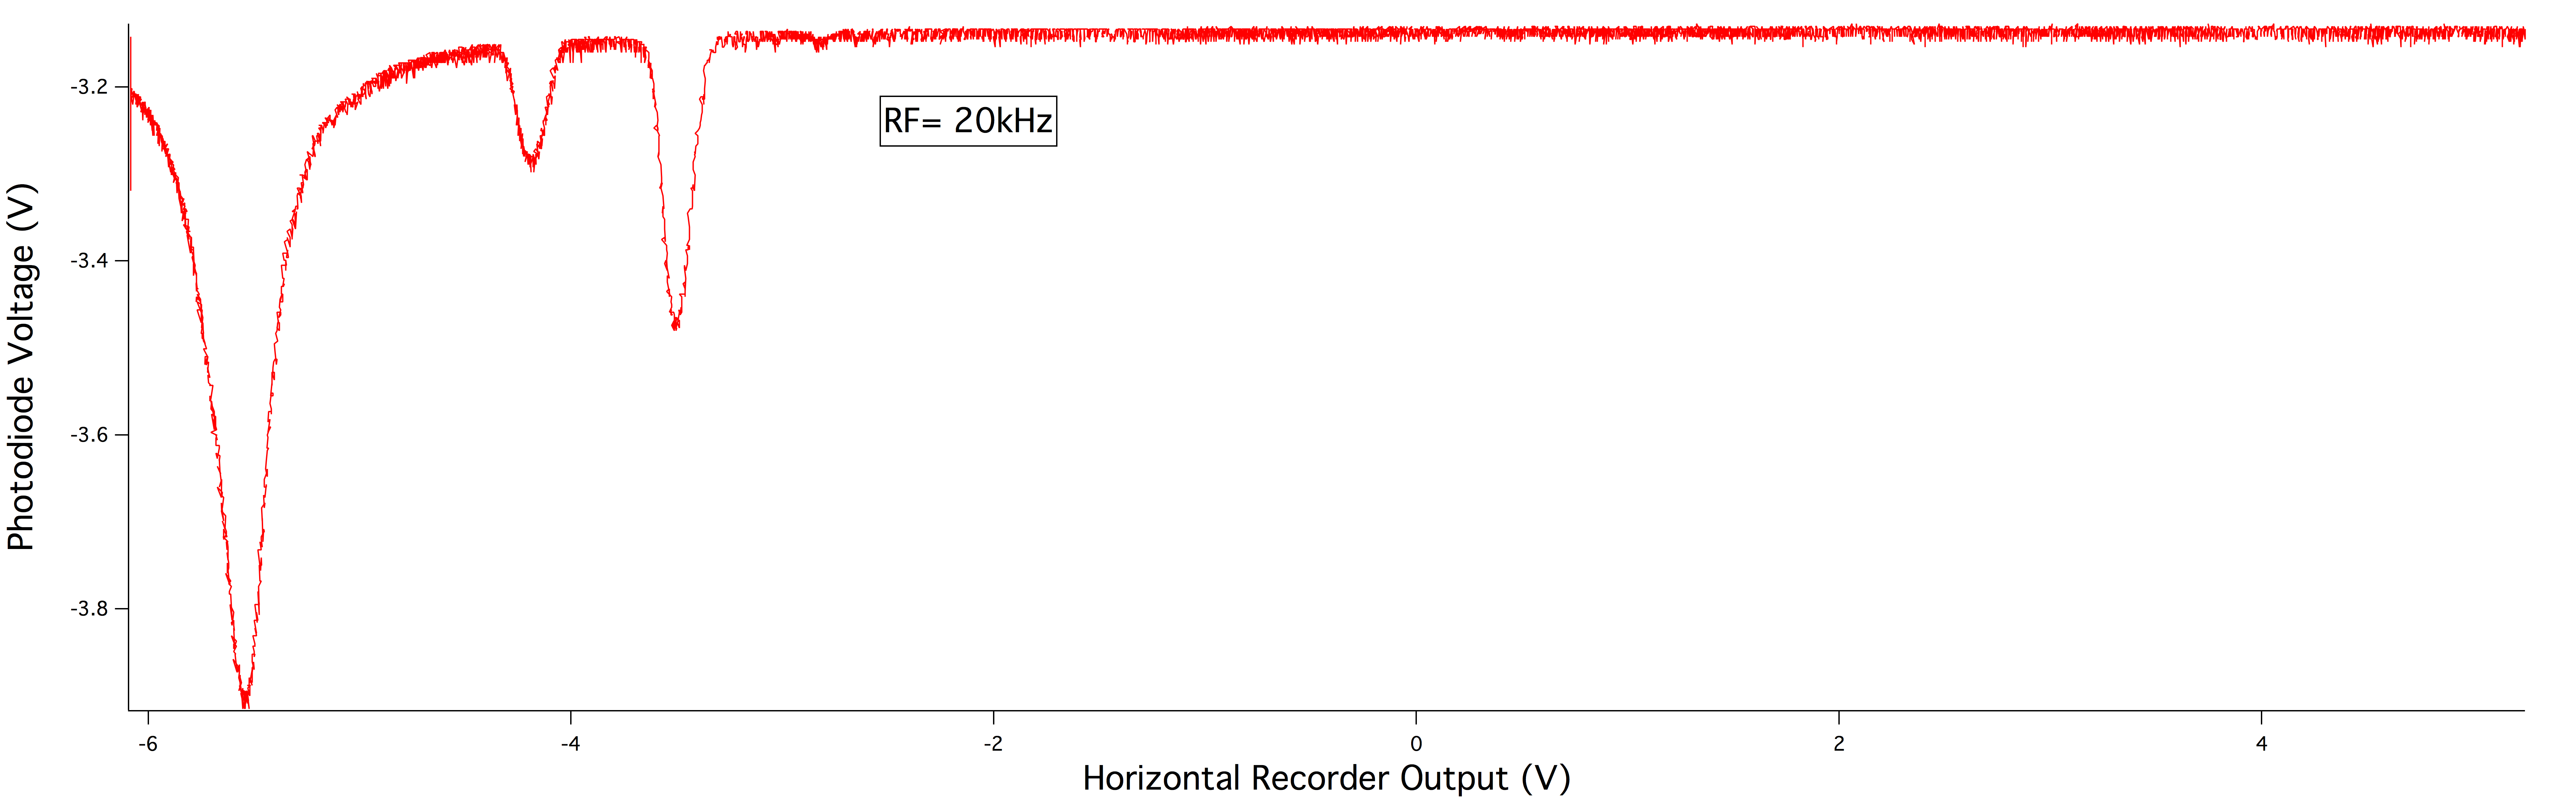
\includegraphics[width=15cm]{20k.png}
\caption{Photodiode voltage versus horizontal recorder output voltage at 100 kHz (top) and 20kHz (bottom). The left trough is the zero field resonance, the middle trough is RF absorption for $^8$$^7$Rb and the right trough is for $^8$$^5$Rb. It is evident that at a higher frequency there is larger  distances between the dips. \textcolor{green}{very nice figure!}}
\label{100kHz}
\end{figure}


Fig. \ref{100kHz} shows two of the ten plots at we made at the ten different frequencies. All ten graphs have similar characteristics where the first dip is where zero field transition occurs when the horizontal field cancels that of the Earth's magnetic field, the first dip is where the  $^8$$^7$Rb transition happens and the second dip is correlated with the $^8$$^5$Rb transition. In the discussion section, we will be using all ten sets of data to find the difference between the zero field transition and the Rb transition is calculated to find the true magnetic field that is resonant with a given RF frequency.\\

The different depth of the dips are caused by different amounts of $^8$$^7$Rb and $^8$$^5$Rb isotopes in nature. There is more $^8$$^5$Rb than $^8$$^7$Rb, which is confirmed by our experiment as the second dip correlated with the  $^8$$^5$Rb transition is deeper. However, the photodiode voltage is not necessary for calculation in this experiment and as we move on to discussion, we will focus more on the location of the dip on the x-axis.\\

%____________Discussion____________________________________________
\section{Discussion}
Voltage is recorded for the horizontal sweep field, but it needs to be converted to magnetic field strength to be useful. The conversion in the unit of Gauss is given by eq.\ref{vtob}
%\vspace*{-0.25cm}
\begin{equation}
B_{\textnormal{sweep}}=8.991\times10^{-3} I N R_{coil}^{-1}
\label{vtob}
\end{equation}
\vspace*{-0.25cm}
where
\vspace*{-0.5cm}
\begin{equation}
I=\frac{V_{\textnormal{sweep}}/{\textrm{Gain}}}{R}
\label{vtoi}
\end{equation}

\textcolor{blue}{The use of words ``Gain'' and ``slope''  rather than symbols such as ``G'' or ``m'' is non-conventional but is OK here if you think it helps avoid confusion with ``g'' and ``M''. Spelling out ``Slope'' would probably be rejected by an actual journal, but it does look better than when it was in italics! } 

$N=11$ is the number of wires wrapped on each side and$R_{coil}=0.1639m$ is the average radius of the loop. Gain is 1 in this experiment and R is the recorder output resistance, which is $30 \Omega$. This is calculated by taking the voltage across the sensor resistor labeled "recorder output" on the horizontal magnetic field sweep on the optical pumping instrument and the monitor voltage, both of which measure the same current passing through the coils. The sweep field voltage is 30 times larger than the monitor voltage, and it is given that the monitor has a sensor resistance of $1 \Omega$. Using Ohm's law of $V=IR$, the resistance of the recorder output is easily found to be $30 \pm ? \Omega $. \textcolor{red}{insert precision in knowledge of \textit{R} here}\\

After converting all the initial voltage values to Gauss using eq.\ref{vtob} and eq.\ref{vtoi}, the x-axis value for all 10 graphs are replaced by the new values in the unit of Gauss. An example of this plot is shown in Fig.\ref{gau}. For all three dips in each graph, a gaussian curve fit is used to find the horizontal field value at the minimum point of the dip. From here, we record the zero field, resonant field for $^8$$^7$Rb and resonant field for $^8$$^5$Rb at all 10 different RF frequencies.\\

\begin{figure}[h]
\centering
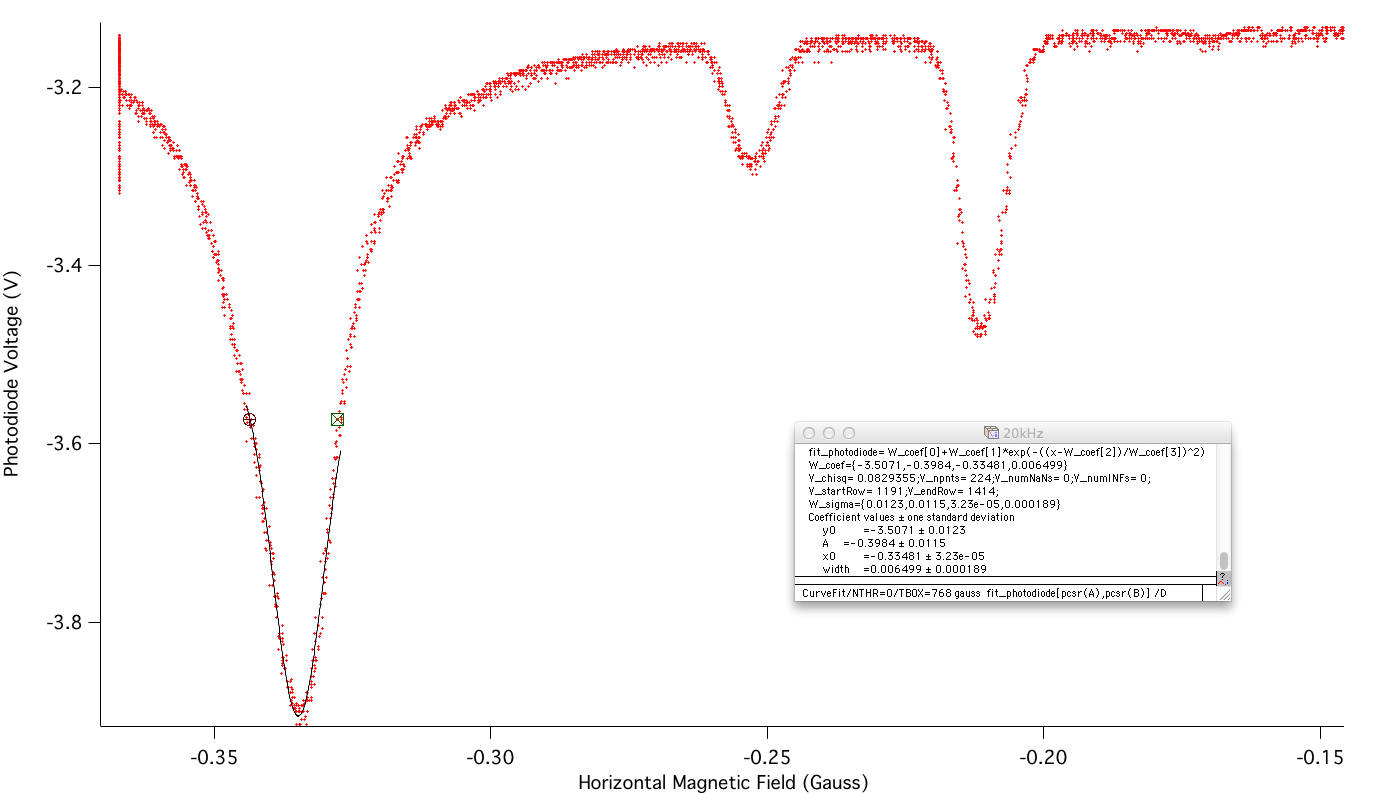
\includegraphics[width=16cm]{gau}
\caption{Using the Gaussian fit to find the horizontal field value, shown on graph annotation as x0, at the zero field dip at RF 20 kHz.}
\label{gau}
\end{figure}


Table.\ref{data} in the appendix shows the positions of all the dips and the resonant fields with uncertainties at the 10 different RF frequencies. The resonant magnetic field is found for both $^8$$^7$Rb and $^8$$^5$Rb at RF frequency varying from 10kHz to 100kHz with a step size of 10kHz, and is also plotted versus the RF frequencies. To find the true resonant fields, the difference between the zero field dips and the resonant dips is calculated and recorded. Table.\ref{data2} shows these new zeroed fields. Using this data, we plotted the new variables in Fig. \ref{both} where it clearly shows the positive linear relationship of the resonant magnetic field and RF frequencies. \\


\begin{figure}[h]
\centering
%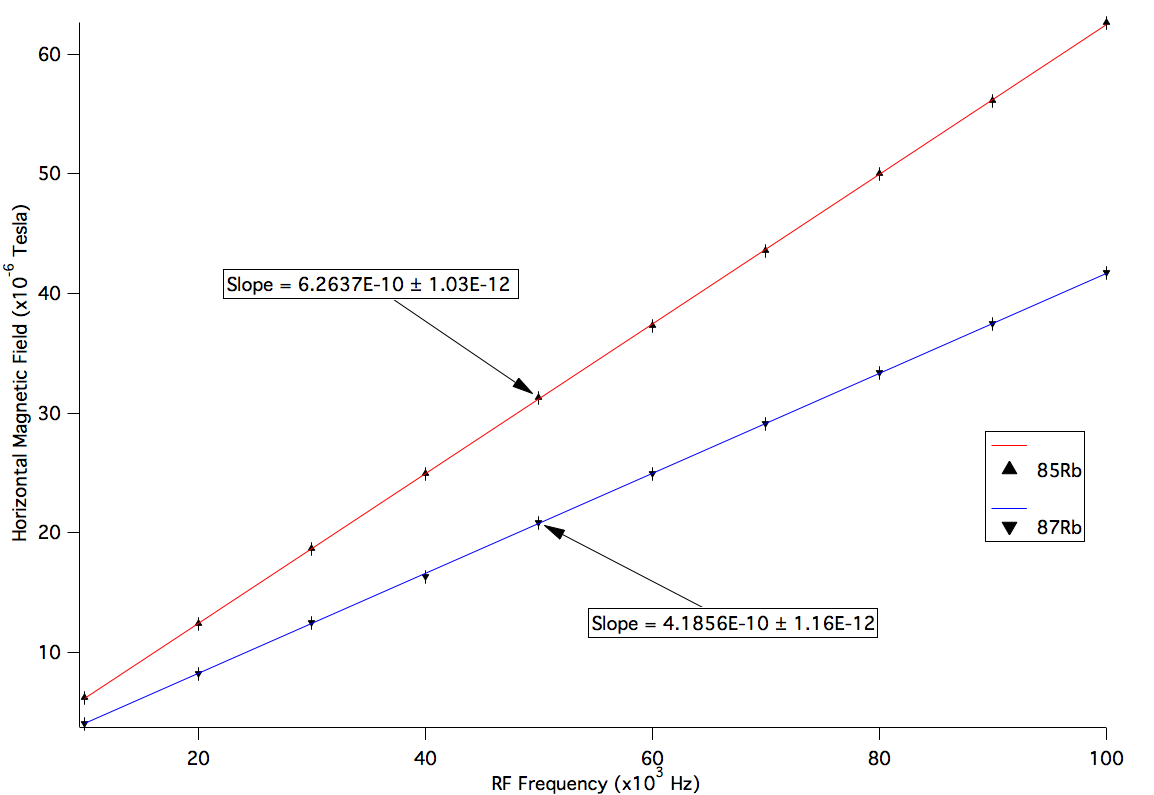
\includegraphics[width=16cm]{both.png}
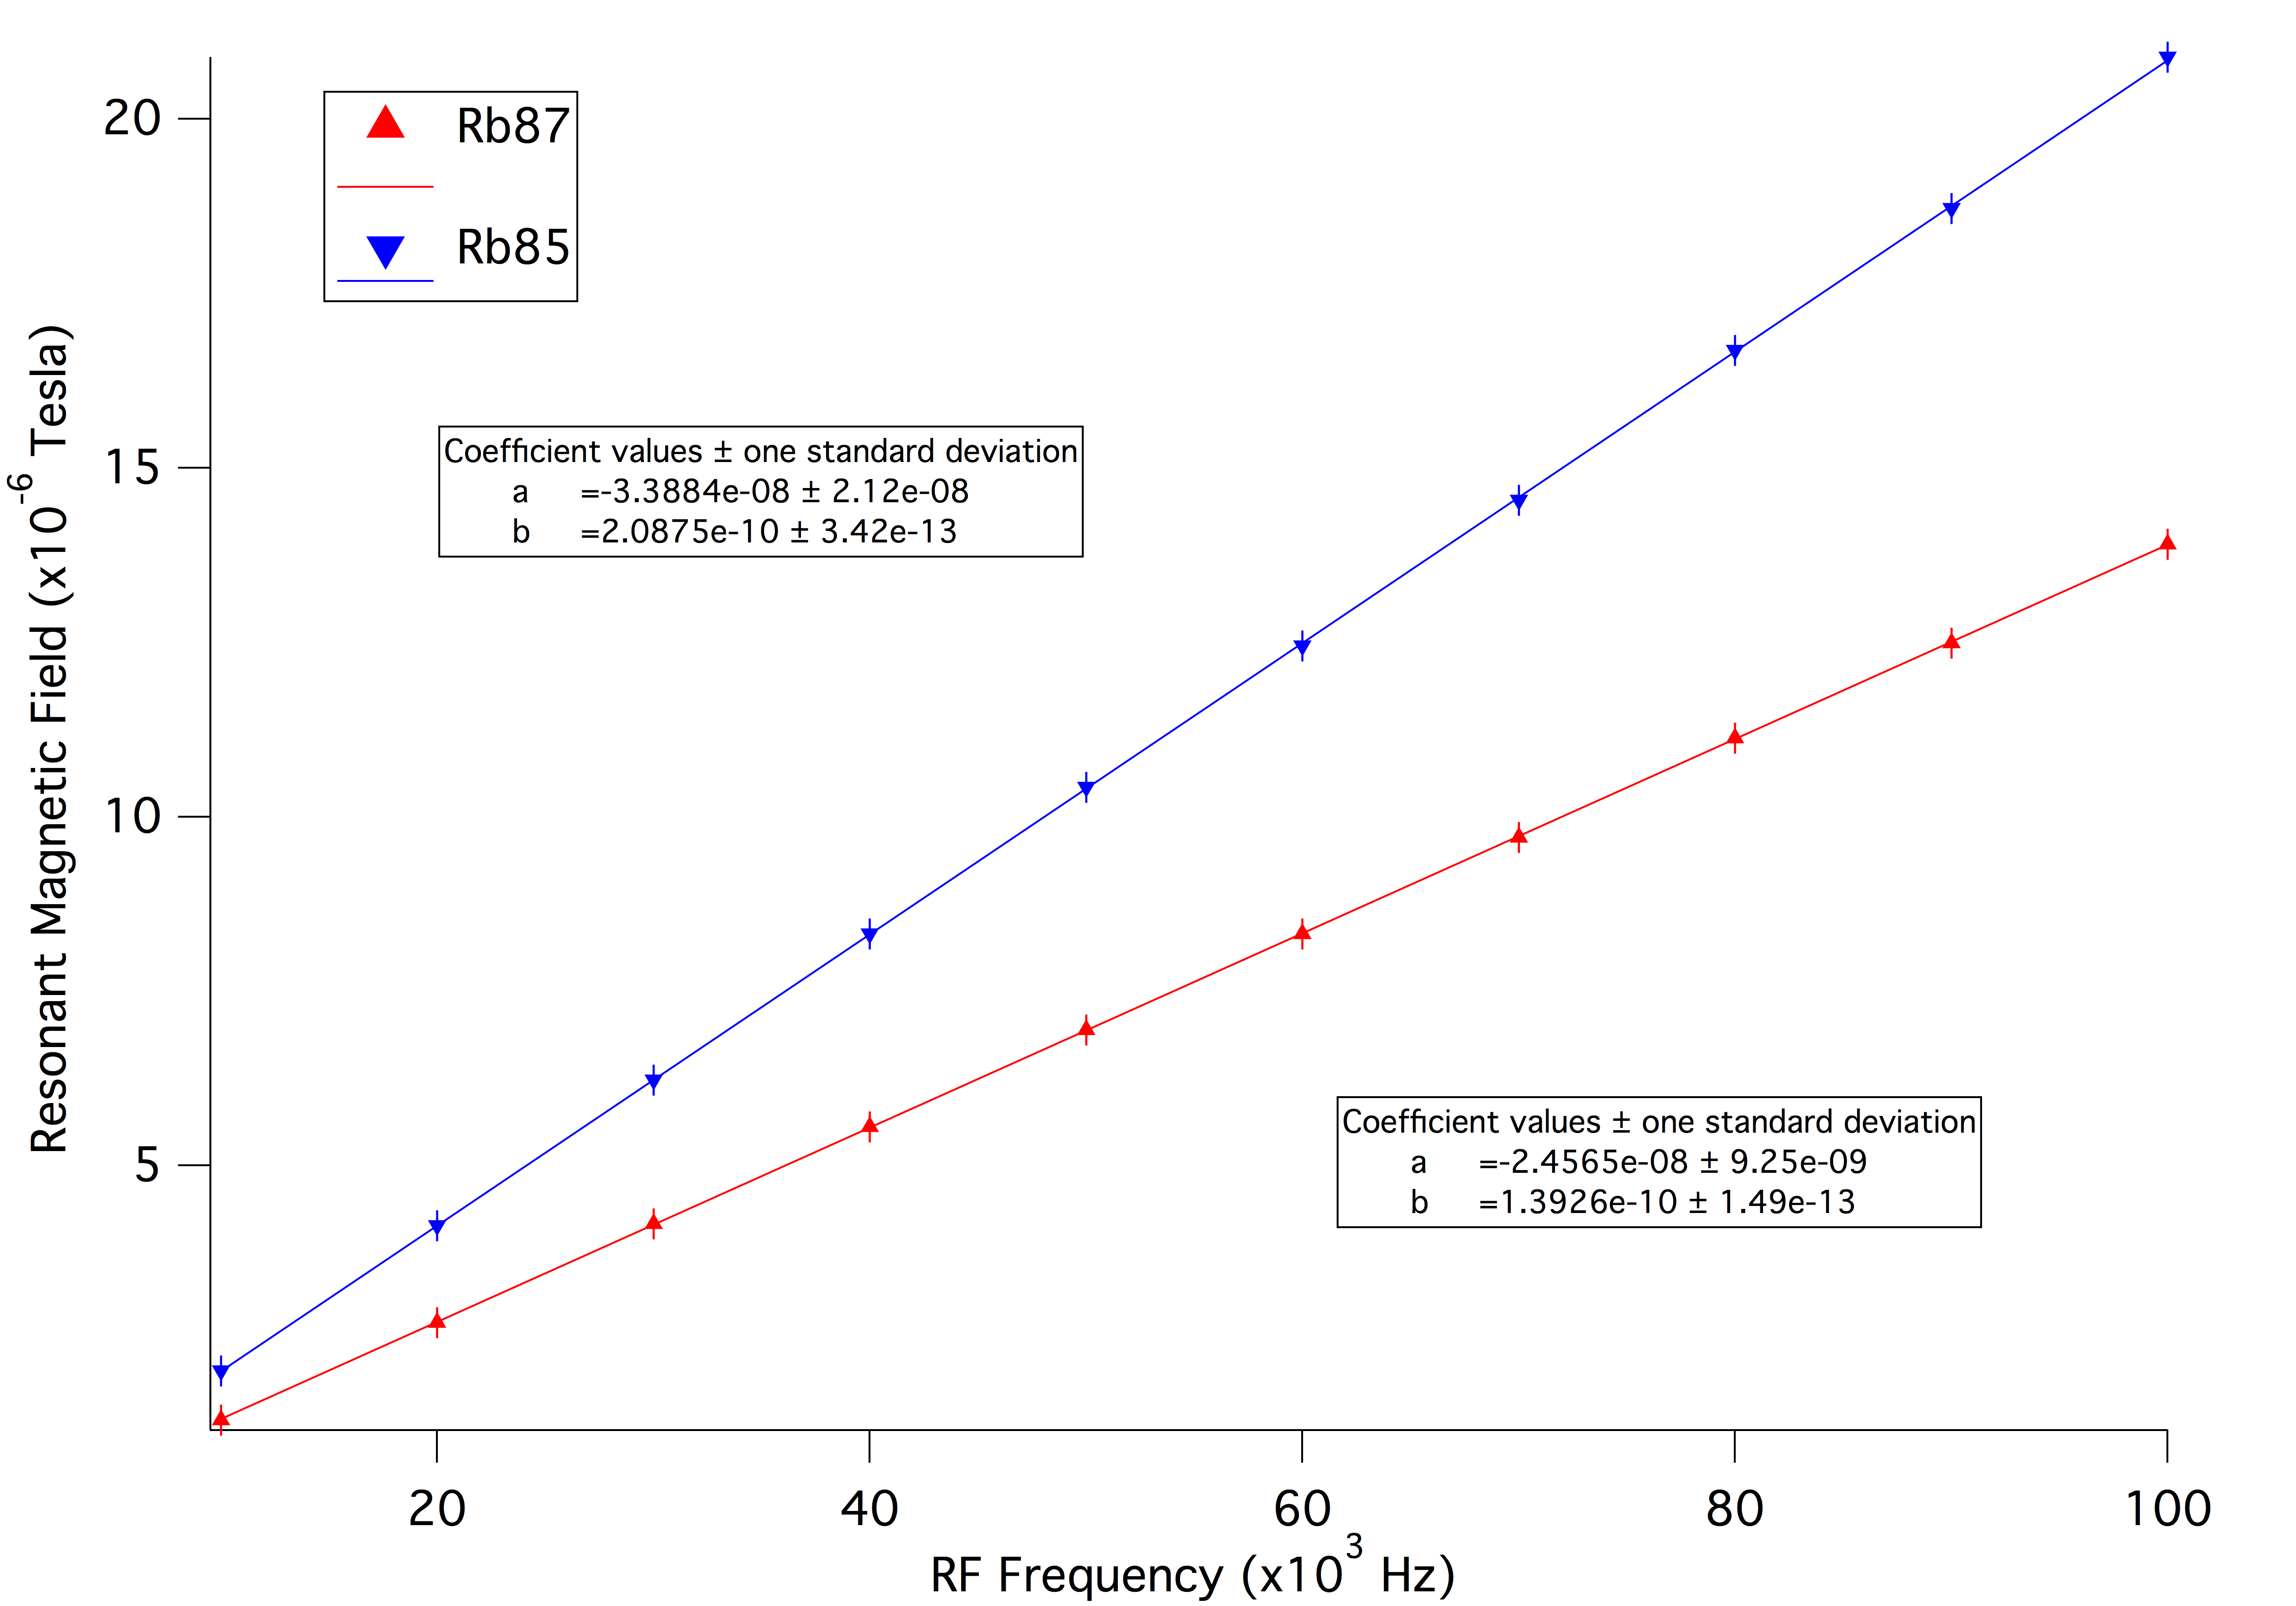
\includegraphics[width=16cm]{slopegraph.png}
\caption{Horizontal magnetic field strength in resonance vs. RF frequency. It is evident that there is a positive linearly proportional relationship between the RF frequency and the resonance field strength. }
\label{both}
\end{figure}

In the plot shown in Fig. \ref{both}, the $^8$$^7$Rb and $^8$$^5$Rb scatter plots are separately fitted by linear curves and their parameters are also shown on Fig.\ref{both} where parameter a is the y-axis intercept and b is the slope of the curve. The slope of the $^8$$^7$Rb is $1.3952\times 10^{-10} \pm 3.88 \times 10^{-13}$ and the slope of the $^8$$^5$Rb is $2.0879 \times 10^{-10} \pm 3.42 \times 10^{-13}$. Resonance only occurs when the RF signal has the right energy to depump the electrons. The "right" energy here is the Zeeman energy, which is the difference in energy between two neighbor $M$ levels. \\

The energy of the RF signal is given by
\begin{equation}
E_{RF}=h\nu
\label{rfenergy}
\end{equation}

Let $E_{RF}=E_{z}$ in Eq. \ref{zeeman} and move the terms around, we get
\begin{equation}
B=\frac{h}{g_{F}\mu_{0}}\nu
\label{bandf}
\end{equation}

where B is the the resonant magnetic field and $\nu$ is the RF frequency. And it is easy to see that they have a linear relationship. $g_{F}$ can be calculate from the slope of the fit line:

\begin{equation}
g_{F}=\frac{\mu_{0}}{h} \times \frac{1}{\textrm{Slope}}=0.51\pm0.0004 \textrm{ for } ^{87}Rb \textrm{ and } 0.34\pm0.0002 \textrm{ for } ^{85}Rb
\label{gf}
\end{equation}


%____________Conclusion____________________________________________
\section{Conclusion}

In this experiment, $g_{F}$ is found to be $0.51\pm0.0004$ for $^8$$^7$Rb and $0.34\pm0.0002$ for $^8$$^5$Rb where the expected values are 1/2 and 1/3. Even though the two expected values are not within the uncertainties of our experimental results \textcolor{blue}{as noted earlier, I am not sure that is the case. I'm not convinced that your precision is to within 0.01\%}, we can see that our values are \textcolor{red}{extremely close} to the theoretical value.

\textcolor{red}{``Extremely close'' is unncessarily vague. be specific. What is the percent deviation between theory and your results?}\\

This experiment could be improved by creating a less magnetically noisy environment. Our experiment was done in a room full of other apparatus and meters, all of which have iron component. Therefore the environmental magnetic field might have influenced our results. Another potential improvement is to align the optical pumping apparatus better with the Earth's magnetic field. We tried to align the apparatus with the compass by inspection. However, the compass was experiencing disturbance when it was close to the apparatus. Therefore our apparatus might not be perfectly aligned, which would introduce an additional magnetic field factor due to the Earth's field into our calculation. \\


%\clearpage

%\vspace*{-2.5cm}

%______________Appendix____________________________________________
\section{Appendix}
%\vspace*{-1.5cm}
\textcolor{blue}{Are you sure you don't mean ``Tesla'' rather than ``Gauss'' in the table below?  Earth's field is on the order of 0.5 Gauss, or 50 microtesla. The horizontal component which you correct for should be on the order of half of that value, or approximately 0.25 G or 24 microtesla. As a result, this table would make a lot more sense if the zero field dip were 33 microtesla rather than 33 microGauss! See also your Figure 5, where you claim the horizontal magnetic field values (after corrections) range from 0 to 20 microtesla. }  
\begin{table}[h]
\centering
\caption{Optical pumping resonance field data}
\begin{ruledtabular}
\begin{tabular}{ l c c c}
RF & Zero Field Dip & Rb87 Dip & Rb85 Dip\\
(kHz) & (\textcolor{red}{Gauss}) & (\textcolor{red}{Gauss}) & (\textcolor{red}{Gauss})\\
\hline
100	& -0.33216$\pm$2.40E-05 & 0.08509$\pm$1.80E-05 & 0.29449$\pm$1.44E-05\\
90&-0.33221$\pm$2.37E-05&0.042623$\pm$2.09E-05&0.22929$\pm$1.61E-05\\
80&-0.33336$\pm$2.79E-05&0.00052957$\pm$1.90E-05&0.16733$\pm$1.23E-05\\
70&-0.33167$\pm$3.33E-05&-0.040531$\pm$2.51E-05&0.10456$\pm$1.51E-05\\
60&-0.33178$\pm$2.96E-05&-0.082066$\pm$2.36E-05&0.041789$\pm$1.62E-05\\
50&-0.33256$\pm$3.65E-05&-0.12408$\pm$2.52E-05&-0.019752$\pm$1.86E-05\\
40&-0.33227$\pm$3.11E-05&-0.16902$\pm$3.25E-05&-0.082741$\pm$2.29E-05\\
30&-0.33257$\pm$3.25E-05&-0.20774$\pm$3.69E-05&-0.1458$\pm$2.44E-05	\\
20&-0.33519$\pm$3.26E-05&-0.2527$\pm$3.73E-05&-0.2111$\pm$2.93E-05\\
10	&-0.335555$\pm$3.79E-05&-0.29493$\pm$7.74E-05&-0.27365$\pm$3.03E-05\\
\end{tabular}
\end{ruledtabular}
\label{data}
\end{table}

\textcolor{blue}{I don't understand the units in Table II. are you saying that at 100 kHz, the resonant field for RB87 is }$13.9 \cdot 10^{-3}$ \textcolor{blue}{tesla}, $13.9 \cdot 10^{-6}$ \textcolor{blue}{tesla}, or $13.9 \cdot 10^{-9}$ \textcolor{blue}{tesla? According to Figure 5, the answer is } $13.9 \cdot 10^{-6}$, \textcolor{blue}{but according to this table, it would be}$(13.9 \cdot10^{-3})(1 \cdot10^{-6}) =  13.9 \cdot10^{-9}$   \textcolor{blue}{tesla}.   
\vspace*{-5cm}

\begin{table}[h]
\centering
\caption{Optical pumping resonance field data (continued)}
\begin{ruledtabular}
\begin{tabular}{ l c c}
RF & RB87 Resonant Field & RB85 Resonant Field\\
(kHz) & ($10^{-6}$Tesla) & ($10^{-6}$Tesla)\\
\hline
100 & 13.908$\pm$1.28E-03 & 20.8883$\pm$1.4E-03\\
90 & 12.4944$\pm$1.33E-03 & 18.7167$\pm$1.49E-03\\
80 & 11.1297$\pm$1.34E-03 & 16.6897$\pm$1.56E-03\\
70 & 9.7046$\pm$1.61E-03 & 14.541$\pm$1.95E-03\\
60 & 8.3238$\pm$1.53E-03 & 12.4523$\pm$1.77E-03\\
50 & 6.9493$\pm$1.84E-03 & 10.4269$\pm$2.06E-03\\
40 & 5.4417$\pm$1.8E-03 & 8.3176$\pm$2.12E-03\\
30 & 4.161$\pm$1.90E-03 & 6.2257$\pm$2.31E-03\\
20 &	2.7497$\pm$2.06E-03 & 4.1363$\pm$2.33E-03\\
10 &	1.3542$\pm$2.27E-03 & 2.0635$\pm$3.84E-03\\
\end{tabular}
\end{ruledtabular}
\label{data2}
\end{table}


\clearpage

\begin{acknowledgments}

We gratefully acknowledge Nathanael Fortune and Dana Parsons, who helped with the experimentation and editing of this experiment.  This work was supported by the Smith College Physics Department.

\end{acknowledgments}


\begin{thebibliography}{99}

\bibitem{teach} TeachSpin Instructions Manual,\textit{Optical Pumping of Rubidium OP1-A}, 6/2002.
\bibitem{rib} Welcome to the University of Minnesota Methods of Experimental Physics Laboratory, http://spa-mxpweb.spa.umn.edu/s11/Projects/S11\_OpticalPumping/apparatus.html,\textit{Optical Pumping of Rubidium}.
\bibitem{energy} Optical Pumping, http://internal.physics.uwa.edu.au/~stamps/2006Y3Lab/SteveAndBlake/theoretical.html

\end{thebibliography}

%\newpage   % Start a new page for tables

\end{document}
